\section{Mise en place CI/CD}
\subsection[Architecture]{Architecture projet}
\begin{frame}{\subsecname}
	Starterkit pour template de site
	 \\
	 module communs
	 \\
	 thème communs
	 \\
	 un site 
	 \\ gros projet de migration de l'existant qui était fait à la bonne franquette
\end{frame}

\subsection{Versions}
\begin{frame}{Gestion de versions}
	Primordial pour différencier les différentes version \\
	avant : manuel \\
	maintenant : auto sur 4 digits. Les deux premiers peuvent être incrémentés auto
\end{frame}

\subsection{Jenkins}
\begin{frame}{\subsecname}
	\missingfigure{Image des jobs jenkins}
	Organisation par portail \\ 
	Job sur SCM \\
	Interaction avec artifactory pour gérer dépôts composer + stocker package \\
	Build continu // Build qualité // release staging / release recette // merge prod
\end{frame}

\subsection{Déploiement}
\begin{frame}{\subsecname}
	build package avec dépendances (expliquer pourquoi)\\
	checksum
	upload
	ansible
	\missingfigure{Récap ansible déploiement}
\end{frame}

\subsection{Sauvegarde}
\begin{frame}{\subsecname}
	TODO activé par une option. choix car staging déploiement fréquent et on ne souhaite pas forcément disposer de backup car environnement de test fréquemment remis à zéro. En recette, option activée. \\ 
	
	Actuellement, restauration manuelle. Prévu de faire un job de restauration.
\end{frame}

\subsection{Monitoring}
\begin{frame}{\subsecname}
	Logs
	Alerte sur Teams (outil com interne) sur les résultats des builds
	\missingfigure{Teams logs}
\end{frame}

\subsection{Sécurité}
\begin{frame}{Sécurité}
	Clés SSH  \\
	Compte nominatif de recette \\
	permissions uniquement pour webserver + user de déploiement. 
	User de déploiement dédié avec droit minimaux (sudo pour seulement quelques commandes)
\end{frame}

\begin{frame}{Bastion}
	\centering 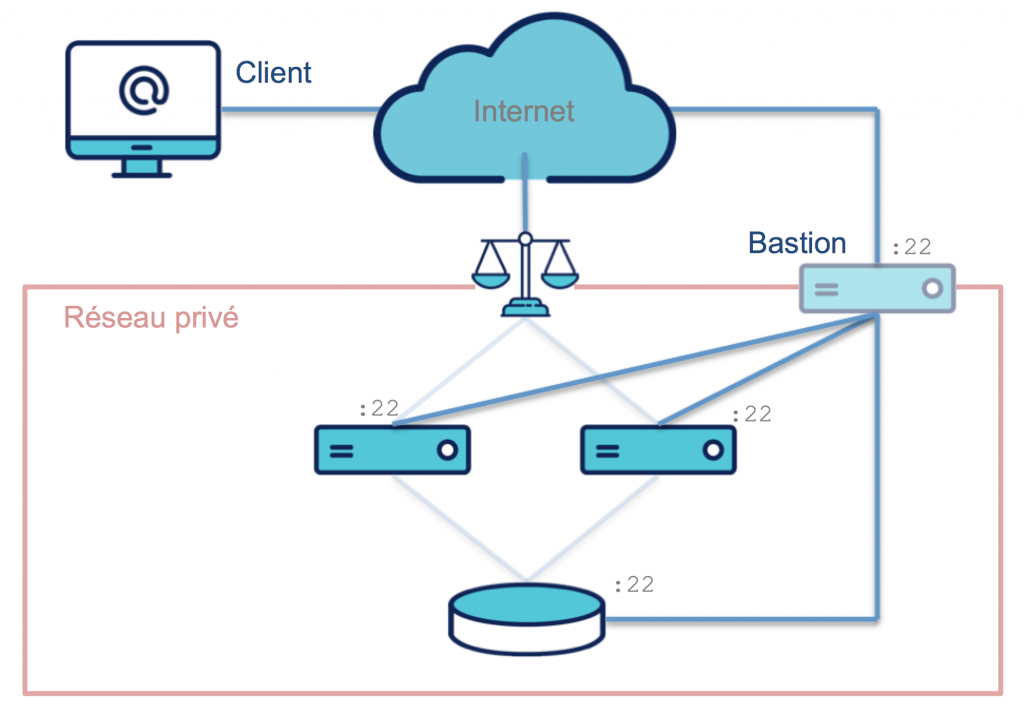
\includegraphics[width=0.60\textwidth]{../img/bastion.png}
\end{frame}
